%! TEX program = xelatex
\documentclass{article}
\usepackage[UTF8]{ctex}
%\usepackage[margin=1in]{geometry}
\usepackage[top=1.5in, bottom=1.5in]{geometry}
\usepackage[hidelinks]{hyperref}
\usepackage{amsmath}
\usepackage{lmodern}
\usepackage{footnote}
\usepackage[bottom]{footmisc}
\usepackage{float}
\usepackage{graphicx}
\usepackage{metalogo}
\usepackage{placeins}
\usepackage{xparse}
\usepackage{listings}
\usepackage{fontspec}
\usepackage{algorithm}
\usepackage{algpseudocode}
\usepackage{caption}

\setmonofont[
    Contextuals={Alternate},
    ItalicFont = Fira Code      % to avoid font warning
]{Fira Code}

\graphicspath{{res/}}

\DeclareDocumentCommand{\inputCodeSetLanguage}{ m }{
    \lstset{
        basicstyle=\small\ttfamily,
        language={#1},
        tabsize=4,
        showstringspaces=false,
        breaklines=true,
        frame=shadowbox,
        framexleftmargin=10mm,
        rulesepcolor=\color{black},
        numbers=left,
        xleftmargin=4em,
    }
}

\NewDocumentEnvironment{simpleAlgorithm}{m}
{
\captionof{algorithm}{#1}
\hrule
\begin{algorithmic}[1]
} {
\end{algorithmic}
\hrule \vspace{1em}
}

%%%%%%%%%%%%%%%%%%%%%%%%%%%%%%%%%%%
%%%%%%%%% BEGIN DOCUMENT %%%%%%%%%%
%%%%%%%%%%%%%%%%%%%%%%%%%%%%%%%%%%%

\title{面向推荐系统的数据挖掘}
\author{计卓1501 胡思勖 U201514898}

\begin{document}
\maketitle

\paragraph{摘要}
\label{par:zhai_yao_}
\par 信息化世界存在着大量的数据,如何在大量的数据中为每一个用户找到其所需求的数据成为了一个问题。本文尝试以包括基于用户的协同过滤算法、基于物品的协同过滤算法以及其混合算法在内的多种不同的推荐算法对于数据进行挖掘分析,并在此过程中尝试对于推荐系统的实现提出一个行之有效的解决方法。

% make paragraph start a new line
\makeatletter
\renewcommand\paragraph{%
    \@startsection{paragraph}{4}{0mm}%
    {-\baselineskip}%
    {.5\baselineskip}%
{\normalfont\normalsize\bfseries}}
\makeatother

\section{综述}
\label{sec:zong_shu_}

\subsection{数据集}
\label{sub:shu_ju_ji_}
\par 本实验采用的数据集使用了Jester数据集\footnote{\url{http://www.ieor.berkeley.edu/~goldberg/jester-data/}}作为所有算法的训练和测试数据集。Jester\footnote{\url{http://eigentaste.berkeley.edu/}}是一个为研究而开发的笑话推荐系统,使用的数据集中的数据则是次系统获取的真实用户数据。
\par 数据集包含3个文件,共包含73,421个用户对于100个笑话的评分数据。数据为xls格式,每一行有101个数据,第一个为用户评价过的笑话个数,剩下的100个为用户对于100个笑话的评分,评分为-10~10之间的实数,99表示``null'',即未打分。数据集的5, 7, 8, 13, 15, 16, 17, 18, 19, 20是密集的,几乎所用的用户都给这些笑话打分过。

\subsection{算法}
\label{sub:suan_fa_}
\par 本次实验采用多种不同的算法并将其结果进行对比。采用的算法包括基于用户的协同过滤算法、基于物品的协同过滤算法等方法。
\par 如图\ref{fig:cf}所示,在协同过滤算法中,用\(m\times n\)的矩阵表示用户对物品的喜好情况,一般用打分表示用户对物品的喜好程度,分数越高表示越喜欢这个物品。图中行表示用户,列表示物品,\(U_{ij}\)表示用户\(i\)对物品\(j\)的打分情况。协同过滤分为两个过程:预测过程和推荐过程。预测过程是预测用户对没有购买过的物品的可能打分值,推荐是根据预测阶段的结果推荐用户最可能喜欢的一个或多个物品。
\begin{figure}[htpb]
    \centering
    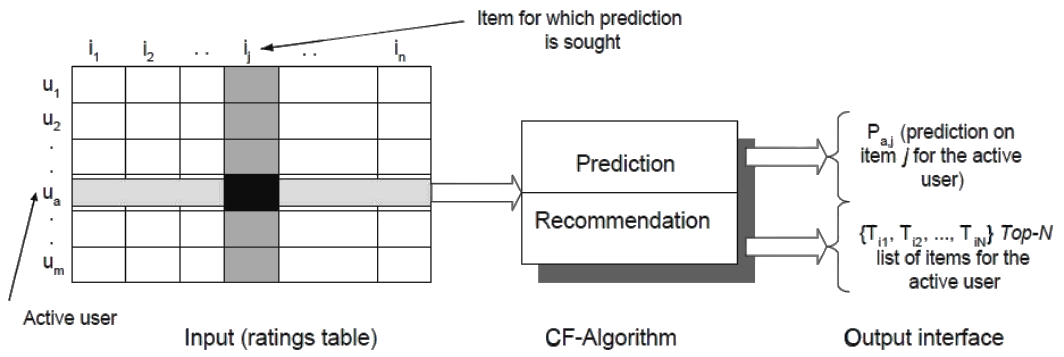
\includegraphics[width=0.9\linewidth]{cf.png}
    \caption{协同过滤算法描述}
    \label{fig:cf}
\end{figure}

\paragraph{基于用户的协同过滤算法}
\label{par:ji_yu_yong_hu_de_xie_tong_guo_lu_suan_fa_}
\par 基于用户的协同过滤算法通过用户的历史行为数据发现用户对商品或内容的偏好,并对这些偏好进行度量和打分。根据不同用户对相同商品或内容的态度和偏好程度计算用户之间的关系。在有相同喜好的用户间进行商品推荐。如图\ref{fig:userBasedCF}所示,如果用户1、用户3两个用户都对于物品2和物品3显示出偏好,并且评价较高,那么用户1和用户3就属于同一类用户,可以将用户1偏好的物品4也推荐给用户3。这里仅是一个简单的例子。在实际的应用过程中还要考虑偏好的程度,同一类用户的人数以及偏好物品的个数等多方面的因素。
\par 简而言之,基于用户的协同过滤算法主要分为2个步骤:
\begin{enumerate}
    \item 寻找相似的用户集合;
    \item 寻找集合中用户喜欢的且目标用户没有的进行推荐。
\end{enumerate}

\begin{figure}[htpb]
    \centering
    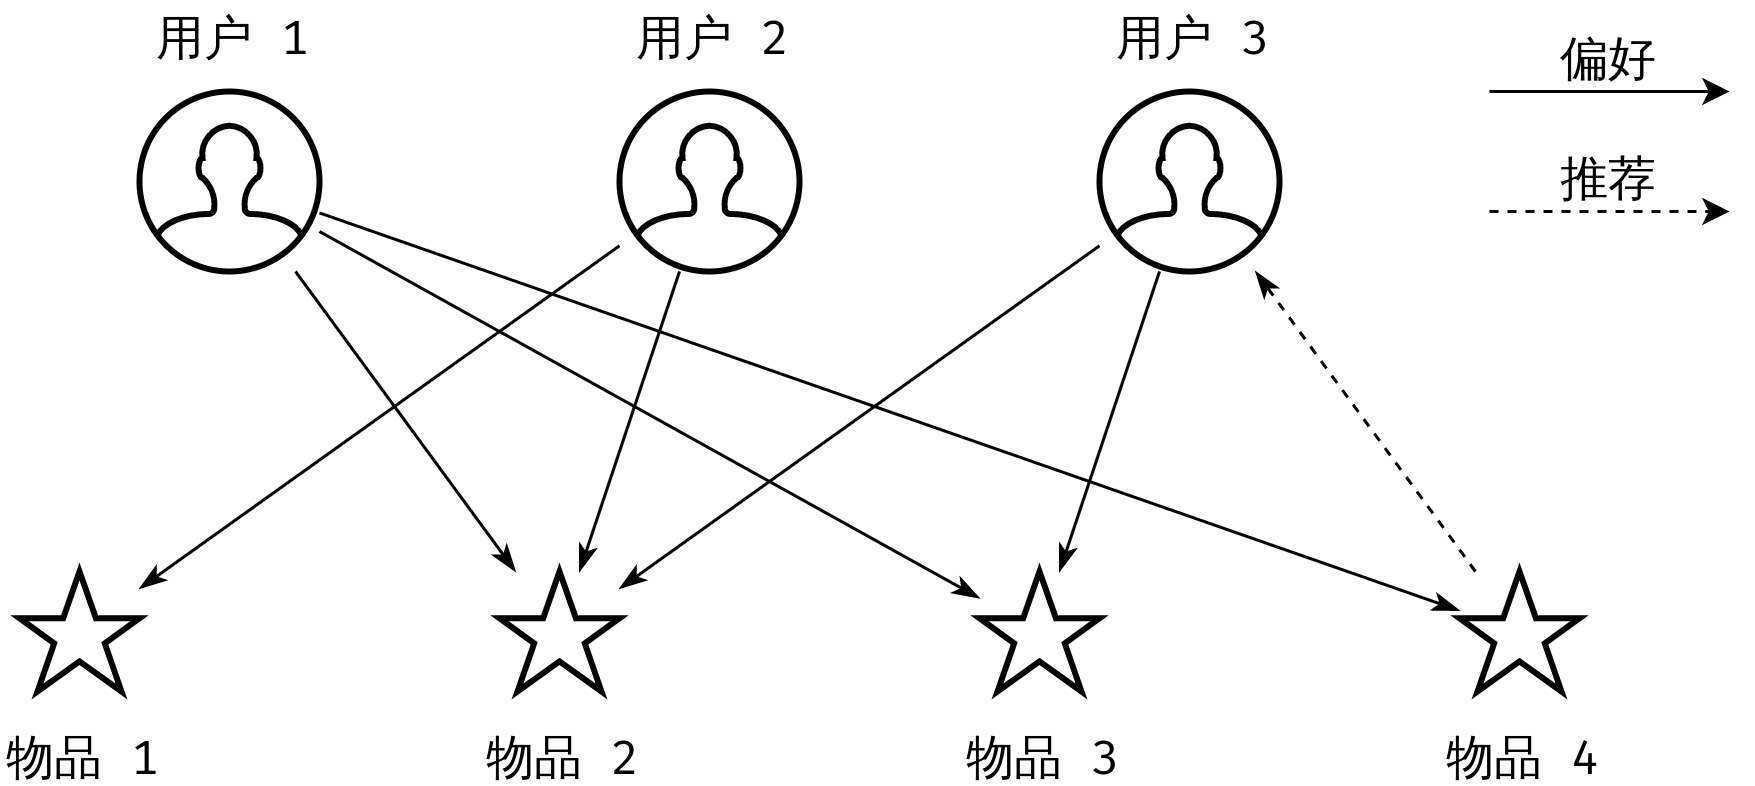
\includegraphics[width=0.8\linewidth]{userBasedCF.png}
    \caption{基于用户的协同过滤算法原理}
    \label{fig:userBasedCF}
\end{figure}
\par 然而,基于用户的协同过滤算法存在两大问题:
\begin{enumerate}
    \item 数据较为稀疏,往往在一个系统中有非常多的物品,而用户偏好的物品数量很少,购买相同物品的用户不够密集,导致无法找到一个用户的邻居进行推荐。
    \item 算法的可扩展性较低,随着用户和物品数量的增加,为所有用户推荐所需时间呈几何模式增加,这往往是一个系统所不能接受的。
\end{enumerate}

\paragraph{基于物品的协同过滤算法}
\label{par:ji_yu_wu_pin_de_xie_tong_guo_lu_suan_fa_}
\par 与基于用户的协同过滤不同,基于物品的协同过滤根据所有的用户偏好计算物品之间的相似度,并把相似的物品推荐给用户。仍以图\ref{fig:userBasedCF}为例,推荐物品2和物品3的人群相似,因此这两个商品相似,在用户2选择物品2时就可以推荐较为相似的物品3。
\par 由于物品间的相似性比较固定,因此可以预先计算不同物品之间的相似度,在性能上较优于基于用户的协同过滤算法。简而言之,基于物品的协同过滤算法分为2步:
\begin{enumerate}
    \item 计算物品之间的相似度;
    \item 根据物品之间的相似度以及用户历史行为给用户生成推荐列表。
\end{enumerate}

% TODO: other algorithms

\par 上述为不同算法的概述,具体的算法实现见第\ref{sec:tui_jian_suan_fa_shi_xian_}节。

\section{数据预处理}
\label{sec:shu_ju_yu_chu_li_}
\par 由于原数据使用99表示用户未平分,而这样的数据在计算时会带来较大的不便,因此在预处理时首先将这些数据置为0,相当于用户在进行-10\textasciitilde 10的连续打分中给这些数据打分为0。可以证明,进行如此的预处理之后在进行各种距离计算时与忽略掉这些数据的结果是一致的,也就是说可以令其直接参与计算而不影响结果。
\par 此外,在使用第三组数据作为训练数据集时,可以考虑预先剔除只给一个物品打分的用户,因为在计算推荐物品时这些用户不可能作出贡献(不可能选择此用户偏好的其他物品进行推荐)。

\section{推荐算法实现}
\label{sec:tui_jian_suan_fa_shi_xian_}

\subsection{基于用户的协同过滤}
\label{sub:ji_yu_yong_hu_de_xie_tong_guo_lu_}

\paragraph{计算用户相似度}
\label{par:ji_suan_yong_hu_xiang_si_du_}
\par 要实现基于用户的协同过滤算法,首先要进行计算的是用户间的相似度。计算用户的相似度主要有4种方法:Jaccard距离、皮尔逊相关系数、闵可夫斯基距离以及余弦距离。其定义分别如下:
\begin{itemize}
    \item Jaccard系数主要用于计算布尔度量的个体间相似度,当个体的特征均使用布尔值进行度量时,无法衡量具体的差异大小,只能获得个体间的特征是否一致,其公式如下:
        \[w_{uv} = \frac{N(u)\cap N(v)}{N(u)\cup N(v)}\]
        其中,\(w_{uv}\)为两个个体之间的相似度,\(N(u)\)和\(N(v)\)分别为\(u\)和\(v\)所具有的属性。
    \item 皮尔逊相关系数是比欧几里德距离更加复杂的可以判断人们兴趣相似度的一种方法。它在数据不是很规范时,会倾向于给出更好的结果。其计算方法如下:
        \[
            \rho_{X,Y} = \frac{cov(X, Y)}{\sigma_x\sigma_y}
            = \frac{E((X - \mu_x)(Y - \mu_y))}{\sigma_x\sigma_y}
            = \frac{E(XY) - E(X)E(Y)}{\sqrt{E(X^2) - E^2(X)}\sqrt{E(Y^2) - E^2(Y)}}
        \]
        其中\(E\)为数学期望,\(cov\)为协方差。
    \item 两个点X和Y之间的闵可夫斯基距离定义为:
        \[\left(\sum_{i=1}^n|x_i - y_i|^p\right)^{\frac{1}{p}}\]
        p取1或2时的闵氏距离是最为常用的,\(p=2\)即为欧氏距离,而\(p=1\)时则为曼哈顿距离。当\(p\rightarrow \infty\)时的极限情况下,可以得到切比雪夫距离:
        \[\lim_{p\rightarrow \infty}\left(\sum_{i=1}^n|x_i - y_i|^p\right)^{\frac{1}{p}} = \max_{i=1}^n |x_i-y_i|\]
    \item 余弦距离,也称为余弦相似度,是用向量空间中两个向量余弦值作为衡量两个个体间差异大小的度量值。欧几里德距离相似,点X、Y的余弦距离表示为:
        \[\text{sim}(X, Y) = \cos{\theta} = \frac{X\cdot Y}{||X||\cdot||Y||}\]
\end{itemize}
\par 在本实验中,由于物品的打分为连续的,为了尽可能的将打分考虑进取以及便于计算,采用余弦距离作为衡量用户之间距离的标准。

\paragraph{推荐算法}
\label{par:tui_jian_suan_fa_}
\par 这里选用了余弦距离作为距离计算方法后,对于任意一个用户\(u\),选取与之\(k\)个用户,用集合\(S(u,k)\)表示,并将\(S\)中所有用户喜欢的物品提取出来,去除目标用户\(u\)已经喜欢的物品。然后对余下的物品进行评分与相似度加权,得到的结果进行排序。最后由排序结果对目标用户\(u\)进行推荐。其中,对于每个可能推荐的物品\(i\),预测的用户\(u\)对其的感兴趣的程度可以用如下公式计算:
\[\hat{r}_{ui} = \frac{\sum_{v\in S(u,K)\cap N(i)} w_{uv}\times r_{vi}}{\sum_{\in S(u,K)\cap N(i)} w_{uv}}\]
其中,\(N(i)\)为对于物品\(i\)打分的用户集合,\(r_{vi}\)为用户\(v\)对于\(i\)的打分,而\(w_{uv}\)为用户\(u\)和用户\(v\)之间的相似程度。
\par 具体的推荐算法如下,传入的参数中,\(item\)为被推荐用户已选物品, \(table\)为训练数据, \(k\)为最近邻居数。

\begin{simpleAlgorithm}{Recommend Algorithm}
    \Procedure{Recommend}{$items, table, k$}
    \State 初始化空堆heap
    \For{\(item\) \textbf{in} \(items\)} \Comment{计算所有用户与当前用户的相似度并入堆}
        \For{\(user\) \textbf{in} 给\(item\)打过分的所有用户}    \Comment{跳过没有交集的用户}
            \If{此用户未计算过}
                \State \(heap\).push({sim(\(items, user\)), \(user\)})
            \EndIf
        \EndFor
    \EndFor

    \State \(nearestUsers \leftarrow \{\}\), \(recommend \leftarrow \{\}\)
    \For{\(i=1\) \textbf{to} \(k\)}  \Comment{找出前k个用户}
        \State nearestUsers.add(\(heap\).pop())
    \EndFor

    \For{\(user\) \textbf{in} \(nearestUsers\)}  \Comment{计算推荐物品以及预测分数}
        \For{\(item\) \textbf{in} \(user\)打分过的物品}
            \If{\(item\) \textbf{in} \(recommend\)}
                \State \(recommend[mi] \leftarrow \sum_{v\in S(u,k)\cap N(i)} w_{uv}\times r_{vi} / \sum_{\in S(u,K)\cap N(i)} w_{uv}\)
            \Else
                \State 更新\(recommend[mi]\)
            \EndIf
        \EndFor
    \EndFor
    \State \Return \(recommend\)
    \EndProcedure
\end{simpleAlgorithm}

\par 在这一算法下,基于训练数据集1的一个可能的推荐列表如图\ref{fig:userOutput}所示,其中包含了这一用户所没有购买的商品推荐及其预测打分(在最终输出中这些分数不会显示,只显示正确率)。
\begin{figure}[htpb]
    \centering
    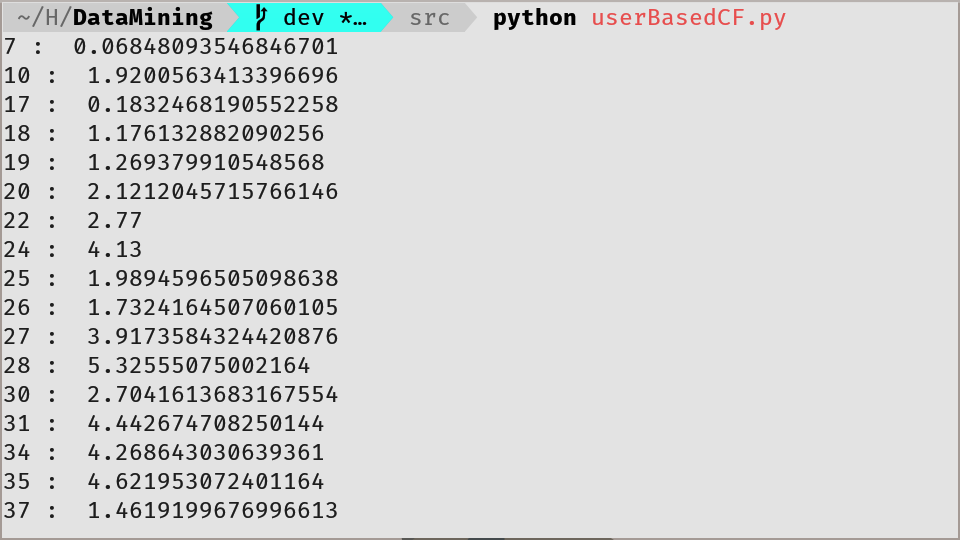
\includegraphics[width=0.9\linewidth]{userOutput.png}
    \caption{一个推荐输出}
    \label{fig:userOutput}
\end{figure}

\subsection{基于物品的协同过滤}
\label{sub:ji_yu_wu_pin_de_xie_tong_guo_lu_}

\paragraph{计算物品相似度}
\label{par:ji_suan_wu_pin_xiang_si_du_}
\par 基于物品的协同过滤相似度计算方法与基于用户的类似,只不过其对象变为了物品,而评估相似度的指标变为了对两个物品进行打分的用户组的相似度。同样,在本实验的相似度计算中采用余弦相似度作为相似度的计算方法。

\paragraph{推荐算法}
\label{par:tui_jian_suan_fa_2}

\par 与基于用户的推荐算法不同,由于本数据集中的物品较少(100个),因此可以先计算物品-物品相似度表,然后通过这一相似度表进行推荐。而对于物品的分数预测方法如下:
\[\hat{P}_{u,i} = \frac{\sum_{i, N}(s_{i,N}\times R_{u, N})}{\sum_{i, N}(|s_{i,N})}\]
其中\(s_{i,N}\)为物品\(i\)与物品\(N\)的相似度,\(R_{u,N}\)为用户\(u\)对于物品\(N\)的打分。此时,基于用户的推荐算法如下,输入参数中items为用户已经打分的物品,而distance为预先计算好的物品相似度表:
\begin{simpleAlgorithm}{Item-Based Recommend Algorithm}
    \Procedure{Recommend}{$items, distance$}
    \State \(recommend \leftarrow \{\}\)
    \For{\(item\) \textbf{in} \(items\)}
        \For{\(otherItem\) \textbf{in} \(distance[item]\)}
            \If{\(item\) \textbf{in} \(recommend\)}
                \State \(recommend[item] \leftarrow \frac{distance[item][otherItem]\times item.score}{distance[item][otherItem]}\)
            \Else
                \State 更新\(recommend[item]\)
            \EndIf
        \EndFor
    \EndFor
    \State \Return \(recommend\)
    \EndProcedure
\end{simpleAlgorithm}
\par 完成算法后,对于随机的一个用户运行程序,得到的输出如图\ref{fig:itemOutput}所示,由于基于物品的协同过滤是对于未选择的物品按序计算的,因此也是按序输出的。
\begin{figure}[htpb]
    \centering
    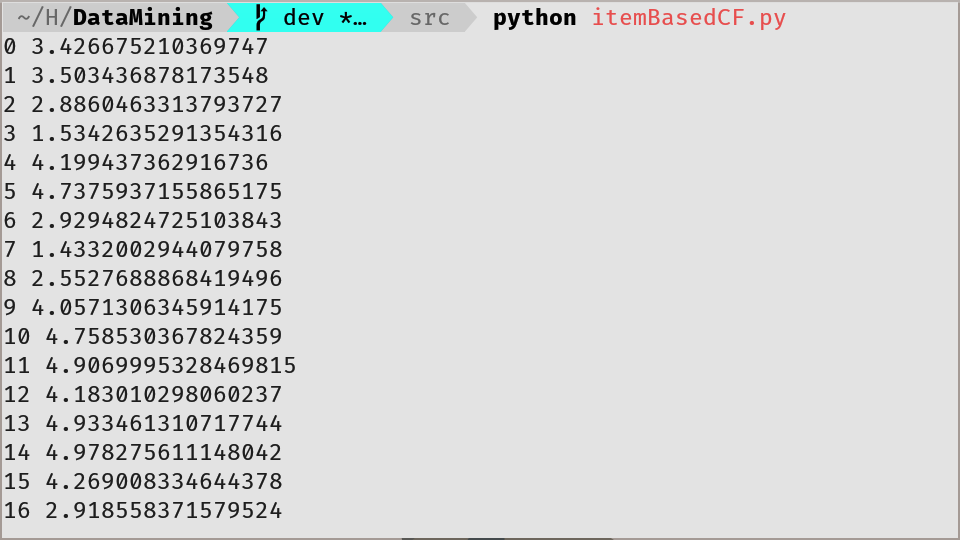
\includegraphics[width=0.9\linewidth]{itemOutput.png}
    \caption{基于用户的协同过滤的一个推荐}
    \label{fig:itemOutput}
\end{figure}

\section{算法测试与结果评估}
\label{sec:suan_fa_ce_shi_}

\subsection{评价指标}
\label{sub:ping_gu_fang_fa_}
\par 要进行完整的测试,需要知道用于评价算法的各个指标。通常而言,用于评价的指标包括:
\begin{itemize}
    \item 准确率: 准确率就是最终的推荐列表中正确的推荐所占有的比例。
    \item 召回率:正确的推荐占全局的比例。
    \item 覆盖率:表示推荐的物品占了物品全集空间的比例。
    \item 新颖度:新颖度是为了推荐长尾区间的物品。用推荐列表中物品的平均流行度度量推荐结果的新颖度。如果推荐出的物品都很热门,说明推荐的新颖度较低,否则说明推荐结果比较新颖。
\end{itemize}
\par 而对于本实验而言,由于打分是连续的,不能简单的判断推荐是否``正确'',因此需要使用其他的方法进行判断。为了能够尽可能准确地评价此推荐系统的准确程度,采用NMAE(Normalized Mean Absolute Error)对于结果进行评价。从Jester数据网站可以得知随机推荐的NMAE约为33\%,而Jester所使用的Egintaste协同过滤算法的准确度为20\%(2000年),以此为基准可以度量本实验所实现的算法的准确性。\newline
\textit{(原文:many papers, including ours, report Normalized Mean Absolute Error (NMAE) rates of approx 20\%. How good is this compared with random guessing? In the Appendix to our paper, we show that if user ratings are uniformly distributed, random guessing yields NMAE = 33\%.)}

\par 除了准确性指标,还需要考虑性能问题,由于基于用户的推荐算法所需要比较的用户数量较多,因此进行推荐的性能可能较差。在这个实验中,通过比较推荐所需的时间(不包含读取与预处理数据的时间)来对于性能进行评估。最终使用的评估算法如下:
\begin{simpleAlgorithm}{Performance Estimation}
    \Procedure{Estimate}{}
    \State \(data \leftarrow\) \Call{readData}{$trainData$}
    \State \(data \leftarrow\) \Call{preProcess}{$data$}
    \State \(testCases \leftarrow\) \Call{readData}{$testData$}
    \State \(testCases \leftarrow\) \Call{preProcess}{$testCases$}
    \State \(avgNMAE \leftarrow 0\)
    \For{\(i=1\) \textbf{to} \(test-case-number\)}
        \State 随机从\(testCases[i]\)中去除部分数据,存入\(testCase\)中
        \State \(result \leftarrow\) \Call{recommend}{$testCase, data$}
        \State \(intersect \leftarrow result\cap testCases[i]\)
        \State \(NMAE_i \leftarrow \frac{\sum_i|result.estimate[i] - result.real[i]|}{N\times (\hat{r}_{max} - \hat{r}_{min})}\)
    \EndFor
    \State \(avgNMAE \leftarrow \frac{\sum_i NMAE_i}{test-case-number}\)
    \EndProcedure
\end{simpleAlgorithm}
\par 其中,\(Recommend\)过程分别选用随机推荐、基于用户的协同过滤以及基于物品的协同过滤以进行比较。

\subsection{评估过程}
\label{sub:ping_gu_guo_cheng_}
\paragraph{在\(测试样例数=500\)的条件下进行测试}
\par 首先进行随机推荐测试,运行randomCF进行推荐,其结果如图\ref{fig:randomOutput}所示,可以看出,NMAE为33.20\%,多次统计结果均在32\%\textasciitilde 34\%之间,由此可以验证上述的``随机推荐NMAE为33\%''这一基准。同时,可以得知使用随机推荐处理1000个用户所需要的时间为0.1秒。

\begin{figure}[htpb]
    \centering
    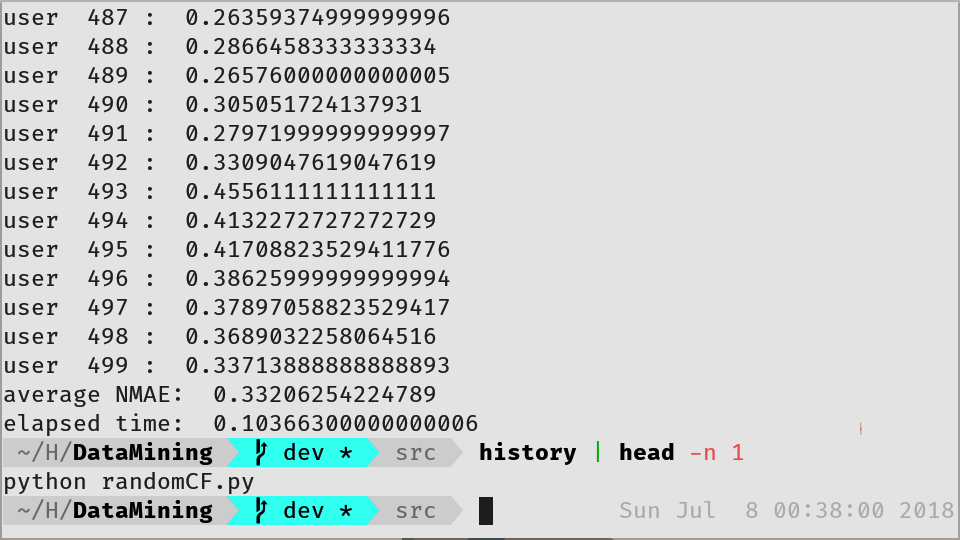
\includegraphics[width=0.9\linewidth]{randomOutput.png}
    \caption{RandomOutput}
    \label{fig:randomOutput}
\end{figure}

\par 接下来,对于基于用户的协同过滤进行测试,测试在同样的条件下进行(输入数据与测试数据相同),在计算相邻用户时取\(k=10\),结果如图\ref{fig:userOutput1}所示。从图中可以看出,推荐的NMAE为22.57\%明显优于随机推荐的33\%,但相比于Egintaste算法的20\%还有较大的改进空间。基于用户的协同过滤用时为197.5秒,约为随机推荐算法的1975倍,说明在用户基数较大时,此算法较为低效。同时,可以看出如对于第499个用户进行推荐时,不能找到有效的推荐,这说明此用户的偏好与其他用户重叠较低,这也是基于用户的协同过滤算法的弊端之一。
\begin{figure}[htpb]
    \centering
    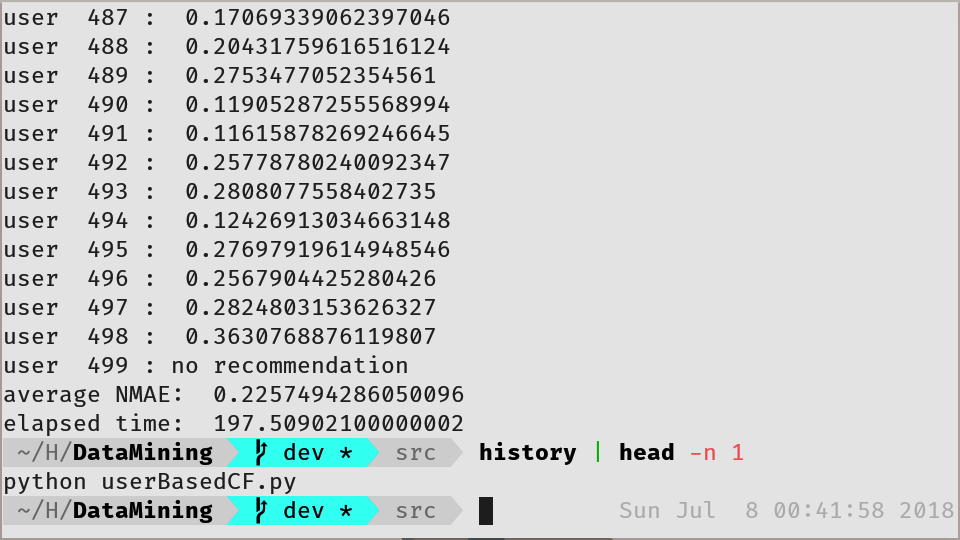
\includegraphics[width=0.9\linewidth]{userOutput1.png}
    \caption{基于用户的协同过滤输出}
    \label{fig:userOutput1}
\end{figure}

\par 最后,对于基于物品的协同过滤进行测试,测试结果如图\ref{fig:itemOutput1}所示,从图中可以看出,对于500个用户推荐仅用时1.65秒,这需要归功于预先建立的物品相似度表。由于此测试数据集的物品较少(只有100件),因而建立的物品相似度表的规模较小。在如电商网站等物品规模持续增大的数据集中,需要采取其他的方法以减少计算的时间。
\par 从图中可以看出,平均NAME达到了18.63,远优于基于用户的协同过滤。同时,由于是计算物品之间的相似度,因此不存在没有近邻而导致的不能推荐的情况,这也可以说明,在这一数据集下,基于物品的协同过滤的整体效果要好于基于用户的协同过滤。

\begin{figure}[H]
    \centering
    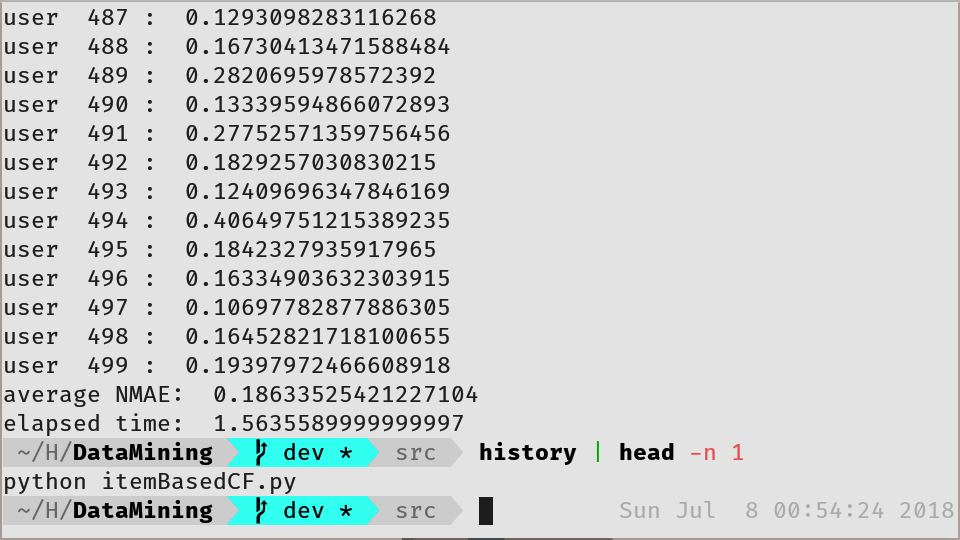
\includegraphics[width=0.9\linewidth]{itemOutput1.png}
    \caption{基于物品的协同过滤输出}
    \label{fig:itemOutput1}
\end{figure}

\subsection{评估结果}
\label{sub:ping_gu_jie_guo_}
\par 除了上述对于基于用户的协同过滤与基于物品的协同过滤的对比外,还需要对于不同的初始值进行计算以评估准确性随着用户已经打过的打分个数的变化。如图\ref{fig:trend}所示,此图使用itemCF中的trend函数生成。其中,横轴为测试样例中已知部分的比例。如\(x=10\)表示已知用户为前10个物品的打分,预测后90个物品的打分,而纵轴为平均NMAE。使用同样的500个样例进行测试。可以发现,在已知打分的占比为50\%\textasciitilde 60\%时预测的准确度最高。

\begin{figure}[htpb]
    \centering
    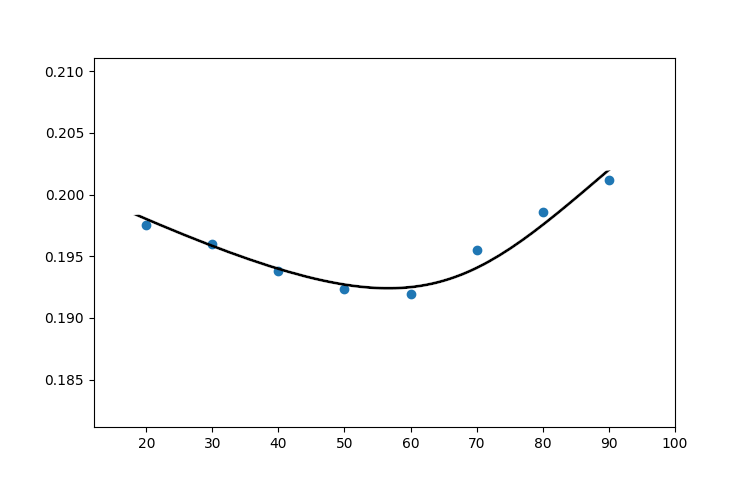
\includegraphics[width=0.9\linewidth]{trend.png}
    \caption{基于物品的协同过滤---NMAE随着已知分数比例的变化}
    \label{fig:trend}
\end{figure}

\par 而对于随机推荐而言,其准确率并不随已知的打分占比明显变化,如图\ref{fig:trendRandom}所示,平均NMAE一直稳定在约33\%的位置。这也与预想的结果一致。将此结果与基于物品的协同过滤结果进行对比,说明已知用户偏好占全部物品的比例小于50\%时预测的准确率呈增加趋势,而大于50\%时呈减少趋势。在实际的应用中,用户观察并评价的物品数一般小于总物品数的50\%,那么在这个区间内,用户评价的越多,推荐就越准确,这也是符合直觉的。然而在物品数较少的情况下就需要考虑当用户评价的物品数占比过大时的``过拟合''状态。此外,从图中可以看到,即使用户的评价很少,NMAE也可以维持在20\%上下,这一结果依旧是十分不错的。
\par 对于基于用户的随机推荐而言,由于计算所花费的时间过长,因此未能生成NMAE岁已知打分比例的变化图,不过根据推测,其趋势应与基于物品的推荐一致。

\par 综上,

\begin{figure}[H]
    \centering
    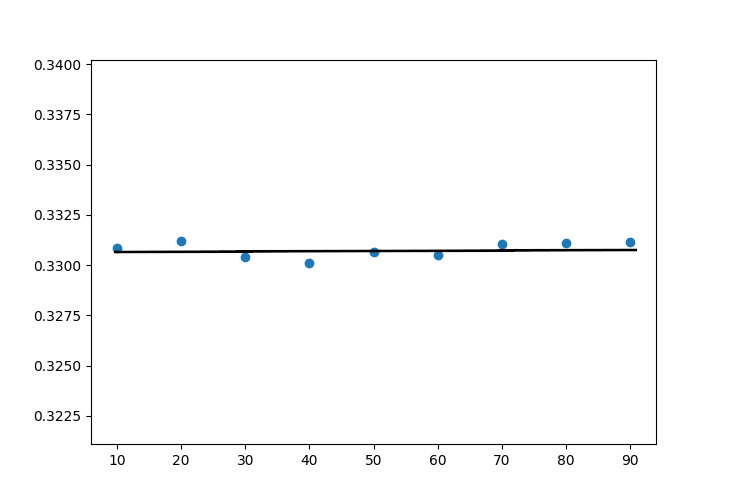
\includegraphics[width=0.9\linewidth]{trendRandom.png}
    \caption{随机推荐---NMAE随着已知分数比例的变化}
    \label{fig:trendRandom}
\end{figure}

% FIXME MAYBE...
%\section{数据可视化}
%\label{sec:shu_ju_ke_shi_hua_}

\section{结语}
\label{sec:jie_yu_}
\par 本实验对于Jester数据集实现了基于用户的协同过滤算法以及基于物品的协同过滤算法,并将其与随机推荐进行比较,同时在基于物品的协同过滤算法上达到了较好的准确性以及性能。
\par 从实验中可以总结,基于用户的协同过滤算法的特点是:
\begin{itemize}
    \item 用户较少的场合,否则用户相似度矩阵计算代价很大;
    \item 适合时效性较强,用户个性化兴趣不太明显的领域;
    \item 对新用户不友好,对新物品友好,因为用户相似度矩阵不能实时计算;
    \item 很难提供令用户信服的推荐解释。
\end{itemize}
对应地,基于物品的协同过滤算法的特点有:
\begin{itemize}
    \item 适用于物品数明显小于用户数的场合,否则物品相似度矩阵计算代价很大
    \item 适合物品丰富,用户个性化需求强的领域
    \item 对新用户友好,对新物品不友好,因为物品相似度矩阵不需要很强的实时性
    \item 利用用户历史行为做推荐解释,比较令用户信服
\end{itemize}
\par 与其他优秀的推荐算法相比(如egintaste、混合算法、基于知识的推荐、基于模型的协同过滤等),本实验中实现的基于物品的协同过滤算法已经达到了较好的效果,但是仍然有较大的改进空间,这主要体现在计算所需要花费的时间上。由于计算各个用户以及各个物品之间的逻辑关联性很小,因此此算法有极大的可并行性,若充分利用多核服务器的并行性能,则能够很好的缩短计算所需要的时间。

\appendix
\section{参考文献}
\label{sec:can_kao_wen_xian_}

\begingroup
\renewcommand{\section}[2]{}%
\nocite{*}
\bibliographystyle{unsrt}
\bibliography{report}
\endgroup

\section{源代码}
\par 此处只给出基于物品的协同过滤的源代码。基于用户的协同过滤以及随机推荐的代码整体框架与之类似,此处不再给出。
\inputCodeSetLanguage{python}
\lstinputlisting{../src/itemBasedCF.py}

\vfill
{\tiny powered by \XeLaTeX \hfill written by 胡思勖}
\end{document}
